\documentclass[11pt, twoside, openright]{book}
\usepackage{jutsu}

\renewcommand{\booktitle}{Deep Reinforcement Learning}
\renewcommand{\booksubtitle}{From Zero to Hero}
\renewcommand{\bookauthor}{Subrat Prasad Panda}
\renewcommand{\bookaffiliation}{NTU Singapore}

\hypersetup{pdftitle={Deep Reinforcement Learning: From Zero to Hero},
            pdfauthor={Subrat Prasad Panda}}

% To compile only the chapter you are working on (much faster), uncomment:
% \includeonly{chapters/01-preliminaries}

\begin{document}

\frontmatter
\makebooktitle

% !TEX root = ../rl_book.tex
\chapter*{Abstract}
\markboth{Abstract}{Abstract}
Lecture notes from for quick revision to RL.

\mbox{}\linebreak
\noindent {\bf Keywords:} Deep Reinforcement Learning $\cdot$ Probability $\cdot$ MDP 


\pdfbookmark{\contentsname}{toc}
\tableofcontents

\mainmatter

% !TEX root = ../rl_book.tex
\chapter{Preliminaries}
\label{chap:preliminaries}

Reinforcement learning draws on several areas of mathematics. This chapter collects the background used throughout the book: probability (\cref{sec:probability}), linear algebra (\cref{sec:linear-algebra}), calculus (\cref{sec:calculus}) and information theory (\cref{sec:information-theory}). Readers comfortable with these topics may skip ahead and return here as needed.

% !TEX root = ../../rl_book.tex
\section{Probability}
\label{sec:probability}

We cover probability with a light touch on measure theory; these notes were prepared while following the lecture series Probability Foundations for Electrical Engineers (IIT M).

\subsection{Introduction}

Probability is the science of randomness that seeks to quantify patterns underlying seemingly non-deterministic events. Andrey Kolmogorov is regarded as the father of modern probability theory. We study probability rigorously because intuitive reasoning can often lead to paradoxes. A famous example is Bertrand’s paradox, where different definitions of “randomness” lead to different probability values. The problem is stated as follows: A chord is drawn at random in a circle. What is the probability that the chord is longer than the side of the equilateral triangle inscribed in the circle? This paradox arises because the sample space is continuous (infinite) and must therefore be defined carefully to avoid ambiguity.

\subsection{Cardinality and Countability}

\subsubsection{Functions and Mappings.}
Given two sets \( A \) and \( B \), a \emph{function} \( f: A \to B \) is a rule that associates every element of \( A \) with a unique element of \( B \).  
The set \( A \) is called the \emph{domain}, and the set \( B \) is called the \emph{codomain}.  
The \emph{range} (or image) of \( f \) is the subset of \( B \) consisting of all elements that are actually mapped to by elements of \( A \), i.e.,
\[
\mathrm{Range}(f) = \{\, f(a) \mid a \in A \,\} \subseteq B.
\]
Note that every element of \( A \) must be mapped to exactly one element of \( B \), although some elements of \( B \) may not receive a mapping from \( A \).

\paragraph{Injective (One-to-One) Function.}
A function \( f: A \to B \) is said to be \emph{injective} if distinct elements of \( A \) map to distinct elements of \( B \). Formally,
\[
f(a_1) = f(a_2) \implies a_1 = a_2, \quad \forall a_1, a_2 \in A.
\]
Equivalently, every element of the range \( \mathrm{Range}(f) \subseteq B \) has a unique preimage in \( A \).

\paragraph{Surjective (Onto) Function.}
A function \( f: A \to B \) is \emph{surjective} if every element of the codomain \( B \) has at least one preimage in \( A \); that is,
\[
\forall b \in B, \; \exists a \in A \text{ such that } f(a) = b.
\]
Hence, for a surjective function, the range equals the codomain: \( \mathrm{Range}(f) = B \).

\paragraph{Bijective Function.}
A function \( f: A \to B \) is \emph{bijective} if it is both injective and surjective.  
In this case, each element of \( B \) has exactly one preimage in \( A \), and \( f \) is said to be \emph{invertible}.  
Its inverse \( f^{-1}: B \to A \) is also a well-defined function satisfying
\[
f^{-1}(f(a)) = a, \quad \forall a \in A, \qquad \text{and} \qquad f(f^{-1}(b)) = b, \quad \forall b \in B.
\]


\subsubsection{Cardinality}

Cardinality is a measure of the ``size'' or number of elements in a set. For finite sets, this is simply the number of elements. However, comparing the sizes of infinite sets is more subtle. For instance, both the set of natural numbers $\mathbb{N}$ and the set of real numbers $\mathbb{R}$ are infinite, yet they are not of the same size. How, then, can we compare their sizes?

\paragraph{Cantor's Argument.}
Two sets have the same cardinality if there exists a bijective (one-to-one and onto) function between them.

\paragraph{Definition.}
Let $A$ and $B$ be two sets.
\begin{enumerate}
    \item $A$ and $B$ are said to have the same cardinality, denoted $|A| = |B|$, if there exists a bijective function $f: A \to B$.
    \item If there exists an injective (one-to-one) function $f: A \to B$ but no bijection, then $B$ has greater or equal cardinality, i.e., $|B| \geq |A|$.
    \item If there exists an injective but not surjective function $f: A \to B$, then $|B| > |A|$.
\end{enumerate}

\paragraph{Theorem.}
The cardinality of the real numbers $\mathbb{R}$ is strictly greater than that of the natural numbers $\mathbb{N}$.

\paragraph{Proof Sketch.}
(Using Cantor's diagonal argument (the ideas to construct new real number by flipping the diagonal entry which will be different from all existing entries).)  
Assume, for contradiction, that there exists a bijection $f: \mathbb{N} \to (0,1) \subset \mathbb{R}$, meaning every real number in $(0,1)$ can be written as a decimal expansion and listed as $f(1), f(2), f(3), \dots$.  
Construct a new real number $r$ by altering the $n$-th digit of $f(n)$ (for instance, replace the $n$-th digit by $5$ if it is not $5$, otherwise by $4$). By construction, $r$ differs from every $f(n)$ in at least one digit, so $r$ is not in the list.  
This contradicts the assumption that $f$ is surjective. Therefore, no bijection exists, and we conclude that
\[
|\mathbb{R}| > |\mathbb{N}|.
\]
Hence, the set of real numbers is uncountably infinite, while the set of natural numbers is countably infinite.


\subsubsection{Countability}

\paragraph{Definition.}
\begin{itemize}
    \item A set $E$ is said to be \textbf{countably infinite} if it is equi-cardinal with $\mathbb{N}$, i.e., there exists a bijection between $E$ and $\mathbb{N}$.
    \item A set is said to be \textbf{countable} if it is either finite or countably infinite.
\end{itemize}

\noindent\textbf{Examples.}
\begin{itemize}
    \item The set of even numbers is equi-cardinal with $\mathbb{N}$ (via $f(n) = 2n$).
    \item The set of integers $\mathbb{Z}$ is countably infinite (we can enumerate them as $0, 1, -1, 2, -2, \ldots$).
    \item The set of rational numbers $\mathbb{Q}$ is also countably infinite.
\end{itemize}

\paragraph{Theorem.}
The set of rational numbers $\mathbb{Q}$ is countably infinite.

\paragraph{Proof Sketch.}
Every rational number can be written as a fraction $\frac{p}{q}$ where $p \in \mathbb{Z}$ and $q \in \mathbb{N}$.  
We can list all such pairs $(p, q)$ in a two-dimensional grid indexed by integers $p$ and positive integers $q$.  
By enumerating these pairs in a diagonal manner (e.g., by increasing $|p| + q$) and skipping equivalent fractions (such as $\frac{1}{2}$ and $\frac{2}{4}$), we can construct a sequence that lists all rational numbers exactly once.  
Thus, there exists a bijection between $\mathbb{Q}$ and $\mathbb{N}$, implying that $\mathbb{Q}$ is countably infinite.  
\[
|\mathbb{Q}| = |\mathbb{N}|.
\]

\paragraph{Note.}
Uncountable sets (such as $\mathbb{R}$) are ``larger'' infinities than $\mathbb{N}$.

\paragraph{Theorem.}
Let $I$ be a countable index set, and let $\{A_i : i \in I\}$ be a collection of countable sets.  
Then the union $\displaystyle \bigcup_{i \in I} A_i$ is countable.  
In other words, a countable union of countable sets is countable.

\paragraph{Proof Sketch.}
For each $i \in I$, enumerate the elements of $A_i$ as $A_i = \{a_{i1}, a_{i2}, a_{i3}, \ldots\}$.  
Arrange these elements in a two-dimensional grid with rows indexed by $i$ and columns by $j$.  
Since both $I$ and each $A_i$ are countable, the set of all pairs $(i,j)$ is countable (using the same diagonal argument as before).  
Now define a mapping from $\mathbb{N}$ to $\bigcup_{i \in I} A_i$ by traversing this grid diagonally and listing each $a_{ij}$ encountered.  
This provides an enumeration of the entire union, proving that
\[
\Big|\bigcup_{i \in I} A_i\Big| = |\mathbb{N}|.
\]
Hence, the countable union of countable sets is countable.

\paragraph{Examples of Countable Sets}
\begin{enumerate}
    \item \textbf{Algebraic Numbers:} The set of all real numbers that are roots of polynomials with integer coefficients. Since each polynomial has finitely many roots, and there are countably many such polynomials, the set of algebraic numbers is countable.
    \item \textbf{Computable Numbers:} The set of all real numbers that can be computed to any desired degree of precision by a terminating algorithm or program. As there are only countably many possible programs, this set is also countable.
\end{enumerate}

\subsubsection{Uncountable Sets}

\paragraph{Definition.}
A set $F$ is said to be \textbf{uncountable} if it has cardinality strictly greater than that of $\mathbb{N}$, i.e., $|F| > |\mathbb{N}|$.  
Equivalently, there exists an injective (one-to-one) mapping from $\mathbb{N}$ to $F$, but no bijection between them.

\paragraph{Examples.}
\begin{itemize}
    \item The set of real numbers $\mathbb{R}$.
    \item The set of irrational numbers $\mathbb{R} \setminus \mathbb{Q}$.
    \item The set of all infinite binary strings $\{0,1\}^{\infty}$.
    \item The power set of the natural numbers $\mathcal{P}(\mathbb{N})$.
\end{itemize}

\paragraph{Theorem.}
The set $\{0,1\}^{\infty}$ of all infinite binary strings is uncountable.

\paragraph{Proof Sketch.}
(Sketch via Cantor’s diagonal argument.)  
Assume that $\{0,1\}^{\infty}$ is countable. Then all binary strings can be listed as:
\[
s_1, s_2, s_3, \ldots
\]
where each $s_i = (s_{i1}, s_{i2}, s_{i3}, \ldots)$ is an infinite sequence of $0$s and $1$s.  
Construct a new binary string $t = (t_1, t_2, t_3, \ldots)$ by flipping the $i$-th digit of $s_i$, i.e.,
\[
t_i = 
\begin{cases}
0, & \text{if } s_{ii} = 1, \\
1, & \text{if } s_{ii} = 0.
\end{cases}
\]
By construction, $t$ differs from each $s_i$ in at least one position (the $i$-th).  
Hence, $t$ is not in the list, contradicting the assumption that the set is countable.  
Therefore, $\{0,1\}^{\infty}$ is uncountable.

\paragraph{Remark.}
To show that another set $A$ is uncountable, it suffices to construct an injective (or bijective) mapping from $\{0,1\}^{\infty}$ to $A$.  
For instance, the interval $[0,1]$ is uncountable because each real number in $[0,1]$ can be represented as an infinite binary sequence.


\subsection{Probability Spaces}

\subsubsection{Random Experiment and Sample Space}

\paragraph{Definition.}
A \textbf{random experiment} is a process that leads to one of several possible outcomes, where the outcome cannot be predicted with certainty in advance.

\paragraph{Sample Space.}
The \textbf{sample space} $S$ (also denoted $\Omega$) is the set of all possible outcomes of a random experiment that we are interested in:
\[
S = \{\text{all possible outcomes}\}.
\]

\paragraph{Example.}
\begin{itemize}
    \item Fair coin toss: coin faces or number of tumbles in air
    \item Velocity with which the coin strikes the ground $\mathbb{R}^+$
\end{itemize}

\paragraph{Remark.}
The definition of $S$ depends on the level of detail we are interested in.
For example, if we include physical parameters of a coin toss (e.g., velocity, angle, or spin), then $S$ may be uncountable. An outcome is denoted by $w \in S$.

\begin{center}
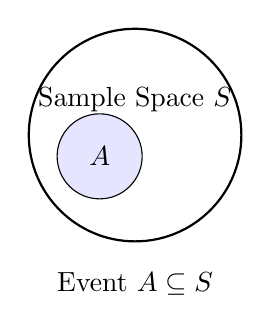
\begin{tikzpicture}[scale=0.9]
\draw[thick] (0,0) circle (1.5);
\node at (0,0.5) {Sample Space $S$};
\draw[fill=blue!10] (-0.5,-0.3) circle (0.6);
\node at (-0.5,-0.3) {$A$};
\node[below] at (0,-1.8) {Event $A \subseteq S$};
\end{tikzpicture}
\end{center}



\subsubsection{Events}

\paragraph{Definition.}
An \textbf{event} is any subset of the sample space $S$ which are of intereset.  
An event occurs if the outcome of the experiment belongs to that subset.

\paragraph{Example.}
When tossing two coins:
\[
S = \{HH, HT, TH, TT\}.
\]
Let $A =$ ``at least one head'' $\Rightarrow A = \{HH, HT, TH\}$.

\paragraph{Note.}
\begin{itemize}
    \item Not all subsets of $S$ are necessarily events (especially in uncountable $S$).
    \item Every event is a subset of $S$.
    \item In uncountable spaces, only measurable subsets are valid events.
    \item some subsets don't behave nicely, so we study it from the lens of measurable space.
\end{itemize}


\subsubsection{Algebra and $\sigma$-Algebra of Events}

\paragraph{Algebra of Sets.}
A collection $\mathcal{F}_0$ of subsets of $S$ is called an \textbf{algebra} if:
\begin{enumerate}
    \item $S \in \mathcal{F}_0$,
    \item If $A \in \mathcal{F}_0$, then $A^c \in \mathcal{F}_0$,
    \item If $A_1, A_2 \in \mathcal{F}_0$, then $A_1 \cup A_2 \in \mathcal{F}_0$.
\end{enumerate}
That is, $\mathcal{F}_0$ is closed under complement and finite unions.

\paragraph{Example.}
Consider tossing a coin until the first head appears.  
Then $S = \{H, TH, TTH, TTTH, \ldots\}$, which is countably infinite.  
The algebra $\mathcal{F}_0$ does not necessarily include infinite unions of its sets.

\paragraph{$\sigma$-Algebra.}
A collection $\mathcal{F}$ of subsets of $S$ is called a \textbf{$\sigma$-algebra} if:
\begin{enumerate}
    \item $S \in \mathcal{F}$,
    \item If $A \in \mathcal{F}$, then $A^c \in \mathcal{F}$,
    \item If $\{A_i\}_{i=1}^\infty \subseteq \mathcal{F}$, then $\bigcup_{i=1}^\infty A_i \in \mathcal{F}$.
\end{enumerate}

\paragraph{Note.}
Every $\sigma$-algebra is also an algebra, but the converse is not true. $\mathcal{F}$ is basically a subset of power-set of $S$.

\noindent
The cardinality of $\mathcal{F}$ could be uncountable, it's matter of how big the uncountable is eg. $2^\mathbb{N}$ vs $2^\mathbb{R}$.



\subsubsection{Measure and Probability Measure}

\paragraph{Measurable Sets.}
Subsets belonging to $\mathcal{F}$ are called \textbf{$\mathcal{F}$-measurable sets}.  
The pair $(S, \mathcal{F})$ is called a \textbf{measurable space}. It is not possile to assing probability to all subsets of power set (with uncountable sample space).

\paragraph{Measure.}
A \textbf{measure} is a function
\[
\mu: \mathcal{F} \to [0, \infty]
\]
that satisfies:
\begin{enumerate}
    \item $\mu(\emptyset) = 0$,
    \item For any countable collection of disjoint sets $\{A_i\}$ in $\mathcal{F}$,
    \[
    \mu\left(\bigcup_{i=1}^\infty A_i\right) = \sum_{i=1}^\infty \mu(A_i).
    \]
\end{enumerate}

The triple $(S, \mathcal{F}, \mu)$ is called a \textbf{measure space}. Space is actualy a set with additional structure.

\paragraph{Types of Measures.}
\begin{itemize}
    \item \textbf{Finite measure:} $\mu(S) < \infty$.
    \item \textbf{Infinite measure:} $\mu(S) = \infty$.
    \item \textbf{Probability measure:} $\mu(S) = 1$.
\end{itemize}


\subsubsection{Probability Measure}

A \textbf{probability measure} $P$ on $(S, \mathcal{F})$ is a function
\[
P: \mathcal{F} \to [0, 1]
\]
such that:
\begin{enumerate}
    \item $P(\emptyset) = 0$,
    \item $P(S) = 1$,
    \item For any countable disjoint collection $\{A_i\} \subseteq \mathcal{F}$,
    \[
    P\left(\bigcup_{i=1}^\infty A_i\right) = \sum_{i=1}^\infty P(A_i).
    \] The summation is monotonically non-decreasing so the sum always converges.
\end{enumerate}

Then $(S, \mathcal{F}, P)$ is called a \textbf{probability space}.  
Elements of $\mathcal{F}$ are the measurable events.

\paragraph{Note.} $\mathcal{F}$ has smaller or equal cardinality than that of power set of $S$. \textbf{Basically, to study probability with nice collection of events.}

\subsubsection{Properties of Probability Measure}

For any events $A, B \in \mathcal{F}$:
\begin{enumerate}
    \item $P(A^c) = 1 - P(A)$
    \item If $A \subseteq B$, then $P(A) \leq P(B)$ (Monotonicity)
    \item $P(A \cup B) = P(A) + P(B) - P(A \cap B)$
    \item Inclusion–Exclusion Principle. For events $A_1, \ldots, A_n$,
\[
P\left(\bigcup_{i=1}^n A_i\right)
= \sum_i P(A_i)
- \sum_{i<j} P(A_i \cap A_j)
+ \sum_{i<j<k} P(A_i \cap A_j \cap A_k) - \cdots
\]
   \item \textbf{Continuity of Probability.} 
    Let $\{A_n\}_{n=1}^\infty \subseteq \mathcal{F}$ be events . Then
    \[
    P\!\left(\bigcup_{n=1}^{\infty} A_n\right) = \lim_{n \to \infty} P(\bigcup_{n=1}^{n} A_n).
    \]
    
    \textbf{Proof Sketch.} 
    Define disjoint sets $B_1 = A_1$, and for $n \ge 2$ let 
    \[
    B_n = A_n \setminus A_{n-1}.
    \]
    Then, $\{B_n\}$ are pairwise disjoint and 
    \[
    \bigcup_{n=1}^{\infty} A_n = \bigcup_{n=1}^{\infty} B_n.
    \]
    By countable additivity,
    \[
    P\!\left(\bigcup_{n=1}^{m} B_n\right) = \sum_{i=1}^{m} P(B_i).
    \]
    Taking the limit as $m \to \infty$ and using monotone convergence,
    \[
    P\!\left(\bigcup_{n=1}^{\infty} A_n\right) 
    = \lim_{m \to \infty} \sum_{i=1}^{m} P(B_i).
    \]
    Thus, the probability measure $P$ is \emph{continuous from below}. 
    Moving the limit outside the measure illustrates the continuity property of $P$.

    
    \item Continuity of Probability (corollary). If $\{A_n\}$ is an increasing sequence of events ($A_1 \subseteq A_2 \subseteq \cdots$), then
\[
P\left(\bigcup_{n=1}^\infty A_n\right) = \lim_{n \to \infty} P(A_n).
\]

    \item If $\{A_n\}$ is decreasing, then
\[
P\left(\bigcap_{n=1}^\infty A_n\right) = \lim_{n \to \infty} P(A_n).
\]
    \item Union Bound: 
   \[
P\!\left(\bigcup_{n=1}^{\infty} A_n\right)
\leq
\sum_{n=1}^{\infty} P(A_n).
\]

\end{enumerate}

\begin{center}
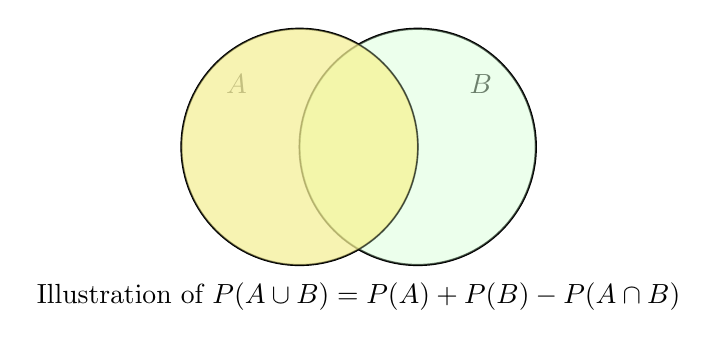
\begin{tikzpicture}[scale=1]
\draw[thick] (0,0) circle (1.5);
\draw[thick] (1.5,0) circle (1.5);
\node at (-0.8,0.8) {$A$};
\node at (2.3,0.8) {$B$};
\node at (0.75,-1.9) {Illustration of $P(A \cup B) = P(A) + P(B) - P(A \cap B)$};
\draw[fill=blue!15, opacity=0.5] (0,0) circle (1.5);
\draw[fill=green!15, opacity=0.5] (1.5,0) circle (1.5);
\draw[fill=yellow!50, opacity=0.6] (0,0) circle (1.5);
\end{tikzpicture}
\end{center}







\subsubsection{Discrete Probability Space}
% Mod 1 Lec 7 https://www.youtube.com/watch?v=PseYlBGV_00&list=PLbMVogVj5nJQqGHrpAloTec_lOKsG-foc&index=7

The discrete space is easy to study since the power set of $S$ contains all measurable sets.
Here, $S$ is countable (finite or countably infinite). Now, we can take set of all events $\mathcal{F}$ as power set $2^{|S|}$ and assign probability to each event. 

If the sample space $S$ is finite or countable, and probabilities are assigned to each outcome $w_i$ such that
\[
P(w_i) \geq 0, \quad \sum_i P(w_i) = 1,
\]
then for any event $A \subseteq S$,
$P(A) = \sum_{w_i \in A} P(\{w_i\})$.
And, $\sum_{w_i \in S} P(w_i) = 1$.

Probabilities are actually assigned to the elements of $\mathcal{F}$ and not to the elements of $S$. However, for discrete case it will be like assigning probability to singleton set ${w} \in \mathcal{F}$. So, $P(w_i)$ is actually $P(\{w_i\})$

How is probability assigned to a singleton set? Since the theory does not prescribe a specific measure for individual singletons, we must determine it empirically through experimentation. Example of assignment if $S=\mathbb{N}$, then $p=1/2^k$ for element $k$ is valid measure (geometric measure). Other measures: Poisson measure.

\subsubsection{Uncountable $S$}

Consider the sample space $S = [0, 1]$, where we imagine throwing a dart uniformly at random onto the line segment. The dart is equally likely to land anywhere between $0$ and $1$, and we wish to assign a **uniform probability measure** on this interval.

However, we cannot assign probabilities to every element of the power set $2^S$. The elementary idea of assigning probabilities to singletons fails in this case: there are uncountably many singleton sets, and summing their probabilities would diverge unless each singleton is assigned probability zero. Moreover, in this continuous setting, we cannot obtain probabilities of intervals simply by adding those of individual points, since the union involved is uncountable.

The key idea is therefore to **abandon the assignment of probabilities to singleton sets** and instead assign probabilities only to more meaningful subsets, such as intervals. The challenge then becomes identifying which subsets should be considered *measurable* and how to assign probabilities to them.

We would like a measure $\mu$ that satisfies the following properties:
\begin{enumerate}
    \item (i) $\mu((a, b)) = \mu([a, b])$, i.e., open and closed intervals have the same measure.
    \item (ii) \textbf{Translation invariance:} $\mu(A) = \mu(A + c)$ for any constant shift $c$, where $A + c = \{x + c : x \in A\}$.
\end{enumerate}

\textbf{Theorem (Impossibility Theorem).}  
There does not exist a measure $\mu(A)$ defined on the full power set $2^S$ (that is, on all subsets of $[0,1]$) satisfying both properties (i) and (ii) for a uniform measure.

Hence, we must **restrict** ourselves to a smaller collection of subsets—those that are still rich enough to include all “interesting” sets like intervals but small enough to admit a consistent measure. This leads to the introduction of the **Borel $\sigma$-algebra**, whose elements, called *Borel sets*, are generated by open intervals through countable unions, intersections, and complements.


\subsection{Generated and Borel $\sigma$-Algebra}

We begin by asking: what should be the smallest $\sigma$-algebra on the real line $\mathbb{R}$?  
We would like to construct a $\sigma$-algebra that contains all intervals and is closed under complementation, countable unions, and intersections.

\paragraph{Generated $\sigma$-Algebra.}
Let $\mathcal{C}$ be an arbitrary collection of subsets of a sample space $S$ (not necessarily a $\sigma$-algebra).  
We aim to construct the smallest $\sigma$-algebra that contains all elements of $\mathcal{C}$.

\begin{definition}[Generated $\sigma$-Algebra]
The \emph{$\sigma$-algebra generated by} $\mathcal{C}$, denoted $\sigma(\mathcal{C})$, is defined as the intersection of all $\sigma$-algebras that contain $\mathcal{C}$:
\[
\sigma(\mathcal{C}) = \bigcap_{\mathcal{F} \supseteq \mathcal{C}} \mathcal{F},
\]
where the intersection is taken over all $\sigma$-algebras $\mathcal{F}$ containing $\mathcal{C}$.
\end{definition}

\begin{theorem}
There exists a smallest $\sigma$-algebra that contains all elements of $\mathcal{C}$.
\end{theorem}

\begin{proof}
Let $\mathfrak{S}$ be the collection of all $\sigma$-algebras that contain $\mathcal{C}$.  
Since the power set $2^S$ is itself a $\sigma$-algebra containing $\mathcal{C}$, the collection $\mathfrak{S}$ is nonempty.  
Define
\[
\sigma(\mathcal{C}) = \bigcap_{\mathcal{F} \in \mathfrak{S}} \mathcal{F}.
\]
The intersection of any family of $\sigma$-algebras is itself a $\sigma$-algebra, hence $\sigma(\mathcal{C})$ is a $\sigma$-algebra that contains $\mathcal{C}$.  
By construction, it is the smallest such $\sigma$-algebra.
\end{proof}

\paragraph{Borel $\sigma$-Algebra.}
If $\mathcal{C}$ is chosen to be the collection of all open intervals in $\mathbb{R}$, then the generated $\sigma$-algebra
\[
\mathcal{B}(\mathbb{R}) = \sigma(\mathcal{C})
\]
is called the \emph{Borel $\sigma$-algebra}.  
It is the smallest $\sigma$-algebra that contains all open intervals of $\mathbb{R}$.  
The sets belonging to $\mathcal{B}(\mathbb{R})$ are called \emph{Borel sets}.



\begin{proposition}
Let $b \in (0,1]$. Then the singleton set $\{b\}$ is a Borel set.
\end{proposition}

\begin{proof}[Proof Sketch]
We can express the singleton $\{b\}$ as a countable intersection of open intervals:
\[
\{b\} = \bigcap_{n=1}^{\infty} (\,b - \tfrac{1}{n},\, b + \tfrac{1}{n}\,).
\]
Since each interval $(b - \tfrac{1}{n},\, b + \tfrac{1}{n})$ is an open set, it belongs to the Borel $\sigma$-algebra.  
Because the Borel $\sigma$-algebra is closed under countable intersections, it follows that $\{b\}$ is a Borel set.
\end{proof}

\paragraph{Examples of Non-Borel Sets.}
While all open, closed, and countable sets are Borel, there also exist subsets of $\mathbb{R}$ that are \emph{not} Borel measurable.  
Famous examples include:
\begin{itemize}
    \item \textbf{Vitali sets} — constructed using the Axiom of Choice by partitioning $\mathbb{R}$ into equivalence classes modulo the rationals.
    \item \textbf{Banach–Tarski paradoxical sets} — subsets of $\mathbb{R}^3$ used in the Banach–Tarski paradox, which demonstrates that certain sets can be decomposed and reassembled into a copy of themselves.
\end{itemize}
These examples highlight the existence of highly non-constructive sets lying outside the Borel $\sigma$-algebra.


\subsubsection{Borel Sets and Lebesgue Measure}

\[
S = (0, 1]
\]
Consider the measure space 
\[
\mathcal{M} = (S, \mathcal{B}),
\]
where $\mathcal{B}$ denotes the Borel $\sigma$-algebra on $S$.  
We aim to define a \emph{uniform measure} on $\mathcal{M}$.

\vspace{0.5em}
\noindent
The intuitive idea is to use \emph{length} as the measure for intervals.  
However, since Borel sets include not only intervals but also more complex (and potentially pathological) subsets, the notion of length must be extended to all elements of $\mathcal{B}$.

\vspace{0.5em}
\noindent
Let $\mathcal{F}_0$ be the collection of all subsets of $S$ that are finite unions of disjoint half-open intervals of the form $(a, b]$, together with the null set.  
For each $A \in \mathcal{F}_0$, we define
\[
\mu(A) = \sum_{i} (b_i - a_i),
\]
where the $(a_i, b_i]$ are the disjoint intervals forming $A$.  
This function $\mu$ represents the intuitive “length” of the set $A$.

\vspace{0.5em}
\noindent
The collection $\mathcal{F}_0$ forms an \emph{algebra} of sets, but it is not a $\sigma$-algebra.  
To obtain a $\sigma$-algebra, we consider
\[
\sigma(\mathcal{F}_0) = \mathcal{B}((0,1]),
\]
the Borel $\sigma$-algebra generated by open (or equivalently half-open) intervals.

\vspace{0.5em}
\noindent
Using the \emph{Carathéodory Extension Theorem}, the measure $\mu$ defined on $\mathcal{F}_0$ can be uniquely extended to a measure on $\mathcal{B}((0,1])$.  
This extended measure is the \emph{Lebesgue measure} restricted to $(0,1]$, and it coincides with our intuitive notion of length on all Borel subsets.

\vspace{0.5em}
\noindent
For example, for any singleton $\{b\} \subseteq (0,1]$, we have
\[
P(\{b\}) = 0,
\]
and for the set of rationals $Q \cap (0,1]$, we also have
\[
P(Q \cap (0,1]) = 0.
\]

\vspace{0.5em}
\noindent
More generally, the Lebesgue measure on $\mathbb{R}$ is denoted by
\[
(\mathbb{R}, \mathcal{B}(\mathbb{R}), \lambda),
\]
where $\lambda$ is infinite and satisfies
\[
\lambda((a,b)) = b - a,
\]
representing the standard notion of length on intervals.

% !TEX root = ../../rl_book.tex
\section{Linear Algebra}
\label{sec:linear-algebra}

\emph{This section is under construction.}

% !TEX root = ../../rl_book.tex
\section{Calculus}
\label{sec:calculus}

\emph{This section is under construction.}

% !TEX root = ../../rl_book.tex
\section{Information Theory}
\label{sec:information-theory}

\emph{This section is under construction.}


% % !TEX root = ../rl_book.tex
\chapter{Introduction}

Reinforcement Learning (RL) is both a problem and solution framework
%studies how an \emph{agent} can learn effective behavior through trial and error while interacting with an \emph{environment}. The agent repeatedly observes, acts, and receives scalar feedback (rewards), and the objective is to learn a behavior that maximizes cumulative reward (the \emph{return}). Deep RL couples these ideas with function approximation via deep networks to represent policies and value functions. \cite{spinningup_rl_intro}

\begin{figure}[h]
\centering
\begin{tikzpicture}[
    >=Stealth,
    looparrow/.style={->, line width=0.9pt, draw=gray!70},
    agentnode/.style={draw, rounded corners=6pt, fill=teal!15, minimum width=3.8cm, minimum height=1.2cm},
    envnode/.style={draw, rounded corners=6pt, fill=blue!10, minimum width=3.8cm, minimum height=1.2cm},
    font=\sffamily
]
  % Nodes
  \node[agentnode] (agent) {Agent};
  \node[envnode, below=10mm of agent] (env) {Environment};

  % Curved arrows with labels
  \draw[looparrow] (agent.east) to [out=0, in=0, looseness=1.25]
    node[midway, right=6mm, align=center] {Action\\$a_t$} (env.east);

  \draw[looparrow] (env.west) to [out=180, in=180, looseness=1.25]
    node[midway, left=7mm, align=center] {State, Reward\\$s_t,\, r_t$} (agent.west);
\end{tikzpicture}

\medskip
\emph{Agent–environment interaction loop.}
\end{figure}


\section{What Can RL Do?}
RL has achieved notable results in game playing (e.g., Go, Dota, Atari), continuous control for robotics (both simulated and real), and instruction-following tasks. These successes illustrate the breadth of domains where learning through interaction and delayed feedback is beneficial. \cite{spinningup_rl_intro}

\section{Key Concepts and Terminology}

\subsection{Agent--Environment Loop}
At discrete time $t=0,1,2,\dots$, the agent receives an observation $o_t$ (often a function of an underlying state $s_t$), selects an action $a_t$, and the environment transitions to $s_{t+1}$ while emitting a reward $r_t$. The goal is to choose actions so as to maximize a cumulative notion of return. \cite{spinningup_rl_intro}

\subsection{States and Observations}
A \emph{state} $s_t$ is a complete description of the world; an \emph{observation} $o_t$ may reveal only part of that state. In deep RL, states/observations are typically represented as real-valued vectors, matrices, or tensors (e.g., pixels for vision, joint angles/velocities for robotics). \cite{spinningup_rl_intro}

\subsection{Action Spaces}
The \emph{action space} may be \emph{discrete} (finite set of actions) or \emph{continuous} (real-valued vectors). This distinction strongly influences algorithm design: many methods are tailored either for discrete or for continuous control. \cite{spinningup_rl_intro}

\subsection{Policies}
A \emph{policy} maps observations or states to actions. Deterministic policies are often written
\[
a_t = \mu_\theta(s_t),
\]
while stochastic policies are written
\[
a_t \sim \pi_\theta(\cdot \mid s_t),
\]
with parameters $\theta$ (e.g., neural network weights) learned by optimization. In practice, categorical policies are common for discrete actions and (diagonal) Gaussian policies for continuous actions. \cite{spinningup_rl_intro}

\subsection{Trajectories}
A \emph{trajectory} (episode) is $\tau=(s_0,a_0,r_0,s_1,a_1,r_1,\ldots)$, generated by rolling out the policy in the environment with its transition dynamics. \cite{spinningup_rl_intro}

\subsection{Reward and Return}
Two standard notions of return are:
\begin{align}
\text{Finite-horizon, undiscounted:}\quad & R(\tau)=\sum_{t=0}^{T} r_t, \\
\text{Infinite-horizon, discounted:}\quad & R(\tau)=\sum_{t=0}^{\infty} \gamma^{t} r_t,\qquad \gamma\in(0,1).
\end{align}
Discounting is both intuitive (earlier rewards count more) and mathematically convenient (guarantees convergence of infinite sums under mild conditions). \cite{spinningup_rl_intro}

\subsection{The RL Objective}
For a policy $\pi_\theta$, the objective is to maximize expected return:
\[
\max_{\theta}\; J(\theta) \;=\; \mathbb{E}_{\tau\sim\pi_\theta}\!\left[\,R(\tau)\,\right].
\]
The expectation is taken over trajectories induced by $\pi_\theta$ and the environment dynamics. \cite{spinningup_rl_intro}

\subsection{Value Functions}
Value functions quantify expected return under a policy $\pi$:
\begin{align}
V^{\pi}(s) &= \mathbb{E}\!\left[ \sum_{t=0}^{\infty}\gamma^t r_t \;\middle|\; s_0=s,\; a_t\sim \pi(\cdot\mid s_t) \right], \\
Q^{\pi}(s,a) &= \mathbb{E}\!\left[ \sum_{t=0}^{\infty}\gamma^t r_t \;\middle|\; s_0=s,\; a_0=a,\; a_{t\ge1}\sim \pi(\cdot\mid s_t) \right].
\end{align}
The corresponding optimal value functions are
\[
V^{*}(s)=\max_{\pi} V^{\pi}(s),\qquad Q^{*}(s,a)=\max_{\pi} Q^{\pi}(s,a).
\]
\cite{spinningup_rl_intro}

There are two key connections between the value function and the action-value function:

\[
V^\pi(s) = \mathbb{E}_{a \sim \pi}[\,Q^\pi(s,a)\,], 
\qquad
V^*(s) = \max_{a} Q^*(s,a).
\]

These follow directly from the definitions:
\begin{itemize}
    \item $V^\pi(s)$ is the expected return starting from $s$ while following $\pi$. Since the first action $a$ is chosen from $\pi(\cdot|s)$, this expectation equals the average of $Q^\pi(s,a)$ under $\pi$.
    \item $V^*(s)$ represents the optimal return achievable from $s$. This is simply the value of the best possible action at $s$, i.e.\ $\max_a Q^*(s,a)$.
\end{itemize}

In the infinite-horizon discounted case, the value function is
\[
V^\pi(s) = \mathbb{E}_\pi \!\left[\sum_{t=0}^\infty \gamma^t r_t \,\Big|\, s_0=s \right],
\]
which depends only on the state $s$ since the problem is stationary and the discount ensures convergence.  

For a finite-horizon undiscounted return
\[
R_t = \sum_{k=t}^{T-1} r_k, \qquad 
V_t^\pi(s) = \mathbb{E}_\pi \!\left[\sum_{k=t}^{T-1} r_k \,\Big|\, s_t=s \right],
\]
the value must depend on time $t$: the same state can have different values depending on how many steps remain. In particular, $V_T^\pi(s)=0$ since no rewards are left once the horizon is reached. Hence, unlike the infinite-horizon discounted case, the finite-horizon setting breaks stationarity and requires $V_t^\pi(s)$.

The optimal action-value function $Q^*(s,a)$ gives the expected return for starting
in state $s$, taking action $a$, and then following the optimal policy thereafter.
The optimal policy selects the action that maximizes this return:
\[
a^*(s) = \arg\max_a Q^*(s,a).
\]
If multiple actions achieve the maximum, any of them is optimal; thus there may be
several optimal policies, but at least one deterministic optimal policy always exists.



\subsection{Bellman Equations}
Value functions satisfy self-consistency (Bellman) relations. For on-policy values:
\begin{align}
V^{\pi}(s) &= \mathbb{E}_{a\sim \pi(\cdot\mid s),\, s'\sim P(\cdot\mid s,a)}\!\left[\, r(s,a) + \gamma V^{\pi}(s') \right], \\
Q^{\pi}(s,a) &= \mathbb{E}_{s'\sim P(\cdot\mid s,a),\, a'\sim \pi(\cdot\mid s')}\!\left[\, r(s,a) + \gamma Q^{\pi}(s',a') \right].
\end{align}
For optimal values:
\begin{align}
V^{*}(s) &= \max_{a}\; \mathbb{E}_{s'\sim P(\cdot\mid s,a)}\!\left[\, r(s,a) + \gamma V^{*}(s') \right], \\
Q^{*}(s,a) &= \mathbb{E}_{s'\sim P(\cdot\mid s,a)}\!\left[\, r(s,a) + \gamma \max_{a'} Q^{*}(s',a') \right].
\end{align}
The right-hand sides are sometimes called \emph{Bellman backups}. \cite{spinningup_rl_intro}

\subsection{Relationship between $V^\pi$ and $Q^\pi$}

The state-value and action-value functions under a policy $\pi$ are related by the following expectation identities:

\paragraph{Expectation over actions (under the policy).}
Since the state-value is the expected return given state $s$, averaging over actions according to the policy,
\begin{equation}
    V^\pi(s) 
    = \mathbb{E}_{a \sim \pi(\cdot|s)}\big[ Q^\pi(s,a) \big]
    = \sum_{a \in \mathcal{A}} \pi(a|s)\, Q^\pi(s,a).
\end{equation}
Here the expectation is taken with respect to the action distribution $\pi(\cdot|s)$.

\paragraph{Expectation over next states (under environment dynamics).}
The action-value is defined as the expected return given state $s$ and action $a$. Using the Bellman equation,
\begin{equation}
    Q^\pi(s,a) 
    = \mathbb{E}_{s' \sim P(\cdot|s,a)}\big[ r(s,a) + \gamma V^\pi(s') \big],
\end{equation}
where the expectation is taken with respect to the next-state distribution 
$P(s'|s,a)$ induced by the environment dynamics.


\subsection{Advantage Functions}
The \emph{advantage} of taking $a$ in $s$ under $\pi$ is
\[
A^{\pi}(s,a) \;=\; Q^{\pi}(s,a) - V^{\pi}(s),
\]
which measures how much better the action is than the policy’s average choice at that state. Advantages are central to many policy-gradient estimators. \cite{spinningup_rl_intro}

\section{(Optional) Formalism: Markov Decision Processes}
A Markov Decision Process (MDP) is a tuple $\langle S,A,R,P,\rho_0\rangle$ with state space $S$, action space $A$, reward function $R:S\times A\times S\to\mathbb{R}$, transition kernel $P:S\times A\to\mathcal{P}(S)$, and initial-state distribution $\rho_0$. The Markov property asserts that $s_{t+1}$ depends only on $(s_t,a_t)$, not on the full past. \cite{spinningup_rl_intro}

\bigskip
\noindent\textbf{Notation.} Throughout, expectations $\mathbb{E}[\cdot]$ are taken over the relevant randomness from the policy and environment; when needed, we use $s'\sim P(\cdot\mid s,a)$ and $a\sim \pi(\cdot\mid s)$ to emphasize sampling.


\begin{figure}[h]
\centering
\begin{tikzpicture}[
  >=Stealth,
  box/.style={draw, rounded corners=6pt, minimum width=4.2cm, minimum height=1.2cm, font=\sffamily, align=center},
  samp/.style={box, fill=orange!15},
  val/.style={box,  fill=blue!12},
  pol/.style={box,  fill=green!15},
  lab/.style={font=\sffamily\footnotesize, align=center}
]

% Nodes arranged in a triangle
\node[samp] (sampling) {Sampling};
\node[val, below right=25mm and -10mm of sampling] (value) {Value Evaluation};
\node[pol, below left=25mm and -10mm of sampling] (policy) {Policy Improvement};

% Curved clockwise arrows
\draw[->, thick] (sampling.east) to [out=0,in=90] node[lab, right=2mm] {trajectories $\mathcal{D}$} (value.north);
\draw[->, thick] (value.south west) to [out=240,in=300] node[lab, below=2mm] {critic / gradients} (policy.south east);
\draw[->, thick] (policy.north) to [out=120,in=180] node[lab, left=2mm] {policy $\pi_\theta$} (sampling.west);

% Notes below each box
\node[lab, below=2mm of sampling] {Collect rollouts with $\pi_\theta$};
\node[lab, below=2mm of value] {Estimate $V^\pi$, $Q^\pi$, $\hat A_t$};
\node[lab, below=2mm of policy] {Update $\theta$ (e.g., PG, PPO, TRPO)};

\end{tikzpicture}

\medskip
\caption{Typical RL algorithm pipeline.}
\end{figure}


\section{Summary}
In value-based reinforcement learning, the error of a $Q$-function update is defined as an 
expectation over the true transition dynamics:
\[
Q(s,a) \;\leftarrow\; r + \gamma \, \mathbb{E}_{s' \sim P(\cdot|s,a)} \big[ \max_{a'} Q(s',a') \big],
\]
where the expectation is taken over the actual environment transition distribution 
$P(s'|s,a)$. 

In contrast, policy-gradient methods shift the focus to the distribution of actions 
induced by the policy:
\[
\nabla_\theta J(\pi_\theta) \;=\; \mathbb{E}_{s \sim d^{\pi}, \, a \sim \pi_\theta(\cdot|s)}
\!\left[ \nabla_\theta \log \pi_\theta(a|s)\, Q^{\pi}(s,a) \right],
\]
where the expectation depends on the state--action distribution under the current 
policy $\pi_\theta$. 

Thus, value-based methods rely directly on transition samples, while 
policy-based methods rely on the action distribution defined by the policy itself.

% % !TEX root = ../rl_book.tex
\chapter{Value-Based Methods}

\section*{Value Iteration and Its Connection to Q-Learning}

A fundamental dynamic programming method in reinforcement learning is
\emph{value iteration}, which computes the optimal value function $V^*(s)$
through repeated application of the Bellman optimality operator:
\[
V_{k+1}(s) = \max_a \Big[ R(s,a) + \gamma \, \mathbb{E}_{s'\sim P(\cdot|s,a)} 
               \big[ V_k(s') \big] \Big].
\]
By iteratively updating all states until convergence, value iteration recovers
$V^*$, and the corresponding optimal policy is obtained by choosing actions
that maximize the one-step lookahead.

Equivalently, one can update action-values via
\[
Q_{k+1}(s,a) = R(s,a) + \gamma \, \mathbb{E}_{s'\sim P(\cdot|s,a)} 
               \big[ \max_{a'} Q_k(s',a') \big],
\]
which directly yields $Q^*(s,a)$ without explicitly maintaining $V$.
This update requires knowledge of the transition dynamics $P(s'|s,a)$ and
reward function $R(s,a)$, and is thus a \emph{model-based} procedure.

\medskip
\noindent
\textbf{Connection to Q-Learning.}  
Q-learning can be understood as a \emph{model-free stochastic approximation} to
value iteration. Instead of requiring expectations with respect to the
transition model, Q-learning uses sampled transitions $(s,a,r,s')$ collected by
interacting with the environment:
\[
Q(s,a) \;\leftarrow\; Q(s,a) + \alpha \Big( r + \gamma \max_{a'} Q(s',a') - Q(s,a) \Big).
\]
This update mirrors the Bellman optimality operator but replaces the
expectation with a single observed transition. As training proceeds, the
estimates $Q(s,a)$ converge toward the optimal action-value function $Q^*(s,a)$
under suitable conditions. Thus, Q-learning can be viewed as the
model-free counterpart of value iteration, extending its principles to
situations where the environment dynamics are unknown and must be learned
purely from interaction.


\section{Deep Q-Network (DQN)}

A landmark in deep reinforcement learning is the Deep Q-Network (DQN) algorithm
\cite{mnih2015human}, which combines Q-learning with deep neural networks.
DQN approximates the optimal action-value function $Q^*(s,a)$ by a parameterized
network $Q_\theta(s,a)$, trained to minimize the Bellman error. A key innovation
was the use of two stabilizing techniques:

\begin{itemize}
    \item \textbf{Experience replay}: transitions $(s,a,r,s')$ are stored in a buffer
    and sampled uniformly for updates, breaking correlations between sequential data.
    \item \textbf{Target networks}: a separate set of parameters $\theta^{-}$ is held
    fixed for computing Bellman targets, updated only periodically, reducing the risk
    of divergence during training.
\end{itemize}

The learned Q-function induces a policy by greedy action selection,
\[
a(s) = \arg\max_a Q_\theta(s,a).
\]

Applied to the Atari 2600 benchmark from raw pixels, DQN demonstrated that a
single agent architecture can learn to play many diverse games directly from
high-dimensional sensory input, achieving performance comparable to or
surpassing human experts on several titles. This result established DQN as a
cornerstone of deep RL and catalyzed much of the subsequent progress in the
field.


% Preamble (once)
% \usepackage{algorithm}
% \usepackage{algpseudocode}
% \usepackage{float}
% \usepackage{amsmath}

\begin{algorithm}[H]
\caption{DQN with Replay, Periodic Batch Updates, and Target Network}
\label{alg:dqn-periodic}
\begin{algorithmic}[1]
\State \textbf{Hyperparams:} replay capacity $N$, batch size $B$, discount $\gamma$, lr $\alpha$
\State \hspace{2.6em} warm-up steps $N_{\text{warm}}$, update period $U$, updates-per-update $K$, target period $C$
\State Initialize replay buffer $\mathcal{D}$ to capacity $N$
\State Initialize Q-network $Q_\theta$ (random $\theta$); target network $Q_{\bar\theta}$ with $\bar\theta \gets \theta$
\For{episode $=1,2,\dots$}
  \State Initialize state $s$ (optionally preprocessed feature $\phi(s)$)
  \While{episode not done}
    \State Select $a$ by $\epsilon$-greedy w.r.t.\ $Q_\theta(s,\cdot)$
    \State Execute $a$; observe $(r, s', d)$ where $d=1$ iff terminal
    \State Push $(s,a,r,s',d)$ into $\mathcal{D}$; set $s \gets s'$
    \State \textbf{(Periodic learning)} \If{$|\mathcal{D}|\ge B$ \textbf{and} $t \ge N_{\text{warm}}$ \textbf{and} $t \bmod U = 0$}
      \For{$k=1$ to $K$} \Comment{$K$ SGD steps per update (UTD)}
        \State Sample minibatch $\{(s_i,a_i,r_i,s'_i,d_i)\}_{i=1}^B \sim \mathcal{D}$
        \State Targets (MSE/Huber loss):
        \[
          y_i \;=\; r_i + \gamma(1-d_i)\,\max_{a'} Q_{\bar\theta}(s'_i,a') 
          \quad\text{\footnotesize (Double DQN: }Q_{\bar\theta}(s'_i,\arg\max_{a'}Q_\theta(s'_i,a'))\text{)}
        \]
        \State $L(\theta)=\tfrac{1}{B}\sum_{i=1}^B \ell\!\big(y_i - Q_\theta(s_i,a_i)\big)$; 
               \quad $\theta \leftarrow \theta - \alpha \nabla_\theta L(\theta)$
      \EndFor
    \EndIf
    \State \textbf{(Target sync)} \If{$t \bmod C = 0$} \quad $\bar\theta \leftarrow \theta$ \EndIf
    \State Increment global step $t \leftarrow t+1$
  \EndWhile
\EndFor
\end{algorithmic}
\end{algorithm}

% !TEX root = ../rl_book.tex
\chapter{Policy Gradient}




\begin{figure}[h]
\centering
\begin{adjustbox}{max width=\linewidth}
\begin{forest}
for tree={
    draw,
    rounded corners,
    align=center,
    inner sep=3pt,
    s sep=8mm,
    l sep=8mm,
    edge={-Stealth},
    font=\small,
    anchor=north,
    minimum width=28mm,
}
[RL Algorithms, fill=blue!10
  [Model-Free
    [Policy Gradient
      [Direct
        [{REINFORCE\\A2C\\A3C}]
      ]
      [Surrogate
        [{PPO\\TRPO}]
      ]
    ]
    [Value-Based
      [Direct
        [DQN]
      ]
      [Critic-Based
        [{DDPG\\SAC\\TD3}]
      ]
    ]
  ]
  [Model-Based
    [Learning Model
      [Dreamer]
    ]
    [Model Given
      [AlphaGo]
    ]
  ]
]
\end{forest}
\end{adjustbox}
\caption{Hierarchy of RL algorithms with grouped methods.}
\end{figure}


% === Policy Optimization with REINFORCE ========
\section{Policy Optimization with \textsc{Reinforce}}

\paragraph{Setup.}
Let $\pi_\theta(a \mid s)$ be a differentiable stochastic policy with parameters $\theta$.
For a trajectory $\tau \!=\! (s_0,a_0,\dots,s_T)$, define the (discounted) return
\[
R(\tau) \;\;=\;\; \sum_{t=0}^{T-1} \gamma^{t}\, r_t,\qquad \gamma\in[0,1].
\]
The performance objective is the expected return
\[
J(\theta) \;\;=\;\; \mathbb{E}_{\tau \sim \pi_\theta}\big[\,R(\tau)\,\big].
\]

\paragraph{Trajectory likelihood and log-derivative trick.}
Under a fixed environment with initial-state distribution $\rho_0$ and dynamics $P$ (both independent of $\theta$),
\[
P(\tau \mid \theta)
\;=\; \rho_0(s_0)\,\prod_{t=0}^{T-1} P(s_{t+1}\mid s_t,a_t)\,\pi_\theta(a_t\mid s_t),
\quad
\log P(\tau \mid \theta)
\;=\; \text{const} + \sum_{t=0}^{T-1}\log \pi_\theta(a_t\mid s_t).
\]
Using $\nabla_\theta P = P \,\nabla_\theta \log P$,
\begin{align*}
\nabla_\theta J(\theta)
&= \nabla_\theta \int P(\tau\mid\theta)\,R(\tau)\,d\tau
= \int P(\tau\mid\theta)\,\nabla_\theta \log P(\tau\mid\theta)\,R(\tau)\,d\tau \\
&= \E_{\tau\sim\pi_\theta}\!\left[\,\sum_{t=0}^{T-1} \nabla_\theta \log \pi_\theta(a_t\mid s_t)\; R(\tau)\,\right].
\end{align*}

\paragraph{Expected Grad-Log-Prob (EGLP) lemma.}
For any distribution $P_\theta$ with density differentiable in $\theta$,
\[
\E_{x\sim P_\theta}\!\big[\nabla_\theta \log P_\theta(x)\big] \;=\; 0.
\]
This follows from $\int \nabla_\theta P_\theta(x)\,dx = \nabla_\theta 1 = 0$.

\paragraph{Reward-to-go form (``don’t let the past distract you'').}
It is preferable to attribute credit to an action only through \emph{subsequent} rewards. Writing
$\hat R_t \coloneqq \sum_{t'=t}^{T-1} \gamma^{t'-t} r_{t'}$,
\[
\nabla_\theta J(\theta)
\;=\;
\E_{\tau\sim\pi_\theta}\!\left[\,\sum_{t=0}^{T-1} \nabla_\theta \log \pi_\theta(a_t\mid s_t)\;\hat R_t\,\right],
\]
which attains lower variance than using $R(\tau)$, since terms involving past rewards cancel in expectation but add noise.

\paragraph{Baselines and advantages.}
By EGLP, for any function $b:\mathcal{S}\!\to\!\mathbb{R}$,
\[
\E_{a_t\sim \pi_\theta(\cdot\mid s_t)}\!\big[\nabla_\theta \log \pi_\theta(a_t\mid s_t)\, b(s_t)\big] \;=\; 0,
\]
so subtracting a baseline does not change the expectation:
\[
\nabla_\theta J(\theta)
\;=\;
\E_{\tau\sim\pi_\theta}\!\left[\,\sum_{t=0}^{T-1} \nabla_\theta \log \pi_\theta(a_t\mid s_t)\,\big(\hat R_t - b(s_t)\big)\right].
\]
The variance-minimizing choice (within state-only baselines) is $b(s_t)=V^{\pi}(s_t)$, yielding the \emph{advantage} $A^{\pi}(s_t,a_t)=Q^{\pi}(s_t,a_t)-V^{\pi}(s_t)$ and the canonical form
\[
\nabla_\theta J(\theta)
\;=\;
\E_{\tau\sim\pi_\theta}\!\left[\,\sum_{t=0}^{T-1} \nabla_\theta \log \pi_\theta(a_t\mid s_t)\, A^{\pi}(s_t,a_t)\right].
\]
In practice, $A^{\pi}$ is estimated from data, e.g., via Monte Carlo $\hat R_t - \hat V(s_t)$ or GAE.

\paragraph{Sample estimator (stochastic gradient).}
Given a batch $\mathcal{D}$ of trajectories sampled under the current policy, with per-time-step weights $w_t \in \{\hat R_t,\;\hat A_t\}$,
\[
\widehat{\nabla_\theta J}(\theta)
\;=\;
\frac{1}{|\mathcal{D}|}\sum_{\tau\in\mathcal{D}}\;\sum_{t=0}^{T-1}
\nabla_\theta \log \pi_\theta(a_t\mid s_t)\; w_t.
\]

\begin{algorithm}[H]
\caption{\textsc{Reinforce} with Reward-to-Go and Baseline}
\label{alg:reinforce}
\begin{algorithmic}[1]
\State \textbf{Input:} policy $\pi_\theta$, critic $\hat V_\phi$, horizon $T$, discount $\gamma$, learning rate $\alpha$
\Repeat
  \State Collect $N$ trajectories by rolling out $\pi_\theta$; store $(s_t,a_t,r_t)_{t=0}^{T-1}$
  \For{each trajectory}
    \State Compute returns-to-go $\hat R_t \gets \sum_{t'=t}^{T-1} \gamma^{\,t'-t} r_{t'}$
    \State (Optional) Estimate advantages $\hat A_t \gets \hat R_t - \hat V_\phi(s_t)$ (or GAE)
  \EndFor
  \State Form policy loss $L(\theta) \gets -\frac{1}{|\mathcal{D}|}\!\sum\limits_{\tau,t} \log \pi_\theta(a_t\mid s_t)\, w_t$
  \State Update policy: $\theta \leftarrow \theta - \alpha\, \nabla_\theta L(\theta)$
  \State (Optional) Update critic $\phi$ by regression to targets $\hat R_t$
\Until{converged}
\end{algorithmic}
\end{algorithm}



\subsection{Generalized Advantage Estimation}

Policy gradient methods rely on the notion of the \emph{advantage function}, defined as
\begin{equation}
    A^\pi(s_t,a_t) = Q^\pi(s_t,a_t) - V^\pi(s_t),
\end{equation}
which measures how much better (or worse) an action $a_t$ is compared to the average behavior at state $s_t$.

\subsection{From Advantage to Temporal-Difference Errors}
Using the Bellman equation for $Q^\pi$, we have
\begin{equation}
    Q^\pi(s_t,a_t) = \mathbb{E}\big[r_t + \gamma V^\pi(s_{t+1}) \mid s_t, a_t\big].
\end{equation}
Substituting into the definition of the advantage,
\begin{equation}
    A^\pi(s_t,a_t) = \mathbb{E}\big[r_t + \gamma V^\pi(s_{t+1}) - V^\pi(s_t) \mid s_t,a_t\big].
\end{equation}
We define the \emph{temporal-difference (TD) error} at time $t$ as
\begin{equation}
    \delta_t = r_t + \gamma V^\pi(s_{t+1}) - V^\pi(s_t).
\end{equation}
Thus, the advantage can be written simply as the expected TD error:
\begin{equation}
    A^\pi(s_t,a_t) = \mathbb{E}[\delta_t \mid s_t,a_t].
\end{equation}

\subsection{Multi-step Advantage Estimators}
Instead of relying only on the $1$-step TD error, one can consider a $k$-step return. Summing discounted TD errors yields
\begin{equation}
    \sum_{i=0}^{k-1} \gamma^i \delta_{t+i} 
    = \Big( r_t + \gamma r_{t+1} + \cdots + \gamma^{k-1} r_{t+k-1} + \gamma^k V(s_{t+k}) \Big) - V(s_t).
\end{equation}
The telescoping structure shows that the $k$-step estimator corresponds to the $k$-step bootstrapped return minus the value baseline.

\subsection{Generalized Advantage Estimation}
Generalized Advantage Estimation (GAE) \cite{schulman2015high} combines all $k$-step estimators into a single exponentially-weighted average:
\begin{equation}
    \hat{A}_t^{\text{GAE}(\gamma,\lambda)} = (1-\lambda)\sum_{k=1}^\infty \lambda^{k-1}
    \left( \sum_{i=0}^{k-1} \gamma^i \delta_{t+i} \right).
\end{equation}
Rearranging terms yields the compact recursive form
\begin{equation}
    \hat{A}_t^{\text{GAE}(\gamma,\lambda)} = \delta_t + \gamma\lambda \delta_{t+1} + (\gamma\lambda)^2 \delta_{t+2} + \cdots.
\end{equation}
In practice, this is implemented efficiently by the backward recursion
\begin{equation}
    \hat{A}_t = \delta_t + \gamma\lambda \hat{A}_{t+1},
\end{equation}
with $\hat{A}_T = 0$ at the end of a trajectory.

\subsection{Bias--Variance Tradeoff}
The parameter $\lambda \in [0,1]$ interpolates between high-bias, low-variance and low-bias, high-variance estimators:
\begin{itemize}
    \item $\lambda=0$: Uses only the $1$-step TD error ($\hat{A}_t=\delta_t$), yielding low variance but higher bias.
    \item $\lambda=1$: Recovers the Monte Carlo return ($\hat{A}_t=R_t - V(s_t)$), yielding low bias but higher variance.
    \item $0 < \lambda < 1$: Provides a balance between variance reduction and bias control, which is crucial for stable policy gradient methods such as PPO and TRPO.
\end{itemize}


\section{Reinforce Extensions}

Algorithms like A2c and A3c

\section{Surrogate Objective}
it covers natural pg, trpo and ppo

\subsection{Surrogate Objective, Natural Gradient, and TRPO}

\paragraph{True objective.}
Let $J(\pi)$ denote the (discounted) expected return of a policy $\pi$:
\[
J(\pi) \;=\; \mathbb{E}_{\tau \sim \pi}\!\left[ \sum_{t=0}^{\infty} \gamma^t r(s_t,a_t) \right],
\quad
d^{\pi}(s) \;=\; (1-\gamma)\sum_{t=0}^{\infty} \gamma^t \Pr(s_t=s \mid \pi)
\]
where $d^{\pi}$ is the discounted state-visitation distribution.

\paragraph{Performance difference and the role of advantages.}
For any two policies $\pi$ and $\pi_{\text{old}}$, the performance difference lemma gives
\begin{equation}
\label{eq:pdl}
J(\pi)
\;=\;
J(\pi_{\text{old}})
\;+\;
\frac{1}{1-\gamma}\;
\mathbb{E}_{s \sim d^{\pi},\, a \sim \pi(\cdot|s)}
\!\big[\, A^{\pi_{\text{old}}}(s,a) \,\big],
\end{equation}
where $A^{\pi_{\text{old}}}(s,a) = Q^{\pi_{\text{old}}}(s,a)-V^{\pi_{\text{old}}}(s)$ is the advantage under $\pi_{\text{old}}$.
Eq.~\eqref{eq:pdl} is exact, but involves the \emph{unknown} distribution $d^{\pi}$ induced by the \emph{new} policy.




\paragraph{From $J$ to a surrogate $L$: switching distributions.}
We would like to evaluate/improve $\pi$ using samples from $\pi_{\text{old}}$.
There are two distributions in \eqref{eq:pdl}:
(i) actions $a \sim \pi(\cdot|s)$ and (ii) states $s \sim d^{\pi}$.

\emph{Action distribution.}
For the inner expectation we use a likelihood-ratio identity:
\[
\mathbb{E}_{a \sim \pi(\cdot|s)}[f(s,a)]
\;=\;
\mathbb{E}_{a \sim \pi_{\text{old}}(\cdot|s)}
\!\left[ \frac{\pi(a|s)}{\pi_{\text{old}}(a|s)}\, f(s,a) \right].
\]

\emph{State distribution.}
Replacing $d^{\pi}$ by $d^{\pi_{\text{old}}}$ yields a tractable, \emph{local} approximation.
This replacement is what makes the objective a \emph{surrogate}: at $\pi=\pi_{\text{old}}$ it matches $J$
to first order (i.e., it has the same gradient), while being computable from data gathered under $\pi_{\text{old}}$.

Putting the two pieces together, the standard surrogate objective around $\pi_{\text{old}}$ is
\begin{align}
\label{eq:surrogate}
L_{\pi_{\text{old}}}(\pi)
&:= J(\pi_{\text{old}})
\;+\;
\frac{1}{1-\gamma}\,
\mathbb{E}_{\substack{s \sim d^{\pi_{\text{old}}}\\ a \sim \pi_{\text{old}}(\cdot|s)}}
\!\left[\, r_{\pi/\pi_{\text{old}}}(s,a)\, A^{\pi_{\text{old}}}(s,a) \,\right],
\\[-2mm]
&\text{with}\quad
r_{\pi/\pi_{\text{old}}}(s,a) := \frac{\pi(a|s)}{\pi_{\text{old}}(a|s)}.
\nonumber
\end{align}
(One often drops the constant $J(\pi_{\text{old}})$ when optimizing, since it does not depend on $\pi$.)


\paragraph{First-order approximation of the surrogate.}
Recall the surrogate objective around $\pi_{\text{old}}$:
\[
L_{\pi_{\text{old}}}(\pi_\theta) 
= J(\pi_{\text{old}})
+ \frac{1}{1-\gamma}\,
\mathbb{E}_{s \sim d^{\pi_{\text{old}}},\, a \sim \pi_\theta(\cdot|s)}
\!\left[ A^{\pi_{\text{old}}}(s,a) \right].
\]

Let $\theta_{\text{old}}$ be the parameters of the current policy and
$\Delta\theta = \theta - \theta_{\text{old}}$ the update.
Performing a first-order Taylor expansion around $\theta_{\text{old}}$ gives
\[
L_{\pi_{\text{old}}}(\pi_\theta)
\;\approx\;
L_{\pi_{\text{old}}}(\pi_{\theta_{\text{old}}})
+ g^\top \Delta\theta,
\]
where
\[
g \;=\; \nabla_\theta L_{\pi_{\text{old}}}(\pi_\theta)\big|_{\theta=\theta_{\text{old}}}
= \mathbb{E}_{s,a \sim \pi_{\text{old}}}
\!\left[ \nabla_\theta \log \pi_\theta(a|s)\, A^{\pi_{\text{old}}}(s,a) \right].
\]

Thus, to first order, maximizing $L$ reduces to taking a step in the
policy gradient direction. This shows that the surrogate objective
recovers the REINFORCE gradient at $\pi = \pi_{\text{old}}$, while also
providing a local approximation of $J(\pi)$ that can be combined with
additional constraints such as a KL trust region.



\paragraph{Why it is a surrogate (first-order accuracy).}
Let $\pi_\theta$ be a differentiable policy, $\theta_{\text{old}}$ the current parameters, and $\Delta\theta=\theta-\theta_{\text{old}}$.
Linearizing $L_{\pi_{\text{old}}}$ at $\theta_{\text{old}}$ gives
\[
L_{\pi_{\text{old}}}(\pi_\theta) \approx L_{\pi_{\text{old}}}(\pi_{\theta_{\text{old}}})
\;+\; g^\top \Delta\theta,
\qquad
g \;=\; \nabla_\theta L_{\pi_{\text{old}}}(\pi_\theta)\big|_{\theta=\theta_{\text{old}}}
= \mathbb{E}_{s,a \sim \pi_{\text{old}}}
\!\left[ \nabla_\theta \log \pi_\theta(a|s)\, A^{\pi_{\text{old}}}(s,a) \right],
\]
which equals the true policy gradient $\nabla_\theta J(\pi_\theta)\!\mid_{\theta=\theta_{\text{old}}}$.
Thus $L$ matches $J$ up to first order at $\theta_{\text{old}}$.

\paragraph{Natural gradient via a local KL constraint.}
To control the size of the update, constrain the average KL divergence from the old policy:
\[
\bar{D}_{\mathrm{KL}}(\theta_{\text{old}},\theta)
\;:=\;
\mathbb{E}_{s \sim d^{\pi_{\text{old}}}}\!\left[
D_{\mathrm{KL}}\!\big(\pi_{\theta_{\text{old}}}(\cdot|s)\,\|\,\pi_{\theta}(\cdot|s)\big)
\right]
\;\le\; \delta.
\]
Approximating the objective to first order and the KL to second order around $\theta_{\text{old}}$ yields
\[
\max_{\Delta\theta}\; g^\top \Delta\theta
\quad \text{s.t.} \quad
\tfrac{1}{2}\,\Delta\theta^\top F\,\Delta\theta \;\le\; \delta,
\qquad
F \;=\; \mathbb{E}_{s,a \sim \pi_{\text{old}}}
\!\big[ \nabla \log \pi_{\theta}(a|s)\, \nabla \log \pi_{\theta}(a|s)^\top \big]_{\theta=\theta_{\text{old}}}.
\]
The solution is the \emph{natural policy gradient} step
\[
\Delta\theta^\star
\;=\;
\sqrt{\frac{2\delta}{g^\top F^{-1} g}}\, F^{-1} g,
\]
which rescales the vanilla gradient by the Fisher information, producing updates that are invariant to reparameterization.

\paragraph{TRPO from the surrogate.}
Trust Region Policy Optimization (TRPO) replaces the linearized objective with the full surrogate \eqref{eq:surrogate}
and enforces the KL constraint directly:
\begin{equation}
\label{eq:trpo}
\max_{\theta}\;\;
\mathbb{E}_{s,a \sim \pi_{\text{old}}}
\!\left[ r_\theta(s,a)\, A^{\pi_{\text{old}}}(s,a) \right]
\quad \text{s.t.} \quad
\mathbb{E}_{s \sim d^{\pi_{\text{old}}}}
\!\left[ D_{\mathrm{KL}}\big(\pi_{\text{old}}(\cdot|s)\,\|\,\pi_\theta(\cdot|s)\big) \right] \;\le\; \delta,
\end{equation}
where $r_\theta(s,a)=\pi_\theta(a|s)/\pi_{\text{old}}(a|s)$.
TRPO approximately solves \eqref{eq:trpo} by computing the natural gradient direction $F^{-1}g$
(via conjugate gradients) and performing a backtracking line search that ensures the empirical KL stays within the trust region
and that the surrogate improves, yielding stable monotonic progress under mild assumptions.

\paragraph{Where the distribution switch occurs.}
The surrogate construction makes two explicit substitutions relative to the true objective:
(i) it \emph{replaces} $d^{\pi}$ by $d^{\pi_{\text{old}}}$ (state distribution switch), and
(ii) it \emph{reweights} the action expectation using the likelihood ratio $r_{\pi/\pi_{\text{old}}}$ (action distribution switch).
These steps allow us to estimate the objective and its gradient from trajectories sampled under $\pi_{\text{old}}$, while the KL trust region controls the discrepancy induced by the state-distribution replacement.





\subsection{Proximal Policy Optimization (PPO)}

Proximal Policy Optimization (PPO) \cite{schulman2017proximal} is an on-policy actor--critic algorithm
designed to improve the stability of policy gradient methods. 
It alternates between (i) collecting trajectories from the current policy and (ii) optimizing a surrogate objective 
over several epochs of minibatch stochastic gradient ascent.

\paragraph{Key ideas.}
\begin{itemize}
    \item The policy $\pi_\theta(a|s)$ (actor) and value function $V_\phi(s)$ (critic) are parameterized by neural networks.
    \item Trajectories of length $T$ are collected, and returns $R_t$ and advantages $A_t$ are computed.
    \item The surrogate objective penalizes large deviations from the old policy via a clipped importance ratio:
    \[
        L^{\text{CLIP}}(\theta) = \mathbb{E}_t\!\left[
            \min\Big(r_t(\theta) A_t,\;
            \mathrm{clip}\!\left(r_t(\theta), 1-\epsilon, 1+\epsilon\right) A_t
            \Big)
        \right],
    \]
    where $r_t(\theta) = \tfrac{\pi_\theta(a_t|s_t)}{\pi_{\theta_{\text{old}}}(a_t|s_t)}$.
    \item The critic is updated by minimizing a squared-error loss 
    $\;L^{\text{VF}}(\phi) = \mathbb{E}_t\!\left[(V_\phi(s_t) - R_t)^2\right]$.
    \item Advantages $A_t$ are estimated using Generalized Advantage Estimation (GAE):
    \[
        A_t = \sum_{l=0}^\infty (\gamma \lambda)^l \delta_{t+l},
        \quad 
        \delta_t = r_t + \gamma V(s_{t+1}) - V(s_t).
    \]
\end{itemize}

\paragraph{Pseudocode.}

\begin{algorithm}[H]
\caption{Proximal Policy Optimization (PPO, clipped variant)}
\begin{algorithmic}
\State Initialize policy parameters $\theta$, value parameters $\phi$
\For{iteration $=1,2,\dots$}
    \State Collect trajectories $\{(s_t,a_t,r_t)\}_{t=0}^{T-1}$ using $\pi_\theta$
    \State Compute returns $R_t$ and advantages $A_t$ (e.g., with GAE)
    \State Store log-probabilities $\log \pi_\theta(a_t|s_t)$ as baseline
    \For{epoch $=1,\dots,K$}
        \State Sample minibatch of transitions
        \State Compute probability ratio $r_t(\theta) \gets \tfrac{\pi_\theta(a_t|s_t)}{\pi_{\theta_{\text{old}}}(a_t|s_t)}$
        \State Compute clipped policy loss $L^{\text{CLIP}}(\theta)$
        \State Update policy by ascending $\nabla_\theta L^{\text{CLIP}}(\theta)$
        \State Update value function by descending $\nabla_\phi L^{\text{VF}}(\phi)$
    \EndFor
\EndFor
\end{algorithmic}
\end{algorithm}

% % !TEX root = ../rl_book.tex
\chapter{Reinforcement Learning Fine-Tuning of Language Models}
\label{chap:rlft}

Notes in this chapter are inspired by the excellent \href{https://youtu.be/BqZC7mDSbIg?feature=shared}{UC Berkeley RL lectures}, which provide a solid foundation for understanding reinforcement learning concepts. We extend these ideas to the modern setting of aligning large language models (LLMs).

\section{Introduction}
Reinforcement Learning Fine-Tuning (RLFT) has emerged as a central paradigm for aligning large language models (LLMs) with human preferences. Unlike classical supervised fine-tuning, RLFT explicitly incorporates feedback (human or automated) to guide the model toward desirable behaviors.  

The three major RLFT approaches are:
\begin{itemize}
    \item Reinforcement Learning from Human Feedback (RLHF, typically implemented with PPO),
    \item Direct Preference Optimization (DPO),
    \item Group Relative Policy Optimization (GRPO).
\end{itemize}

Each method differs in how it incorporates preference information, but they share a common principle: moving the model distribution closer to human-preferred behaviors while avoiding divergence from the reference distribution.

The overall training pipeline can be summarized as follows:
\begin{enumerate}
    \item \textbf{Pre-training:} Train the LLM on internet-scale corpora with next-token prediction.
    \item \textbf{Supervised Fine-Tuning (SFT):} Use human-annotated demonstrations to fine-tune the model. However, labeled data is limited, and imitation alone is insufficient for robust generalization.
    \item \textbf{Reinforcement Learning Fine-Tuning:} Collect preference data by sampling multiple completions for a given prompt and asking a judge (human or automated) to indicate preferred outputs. This preference data is then used to fine-tune the model, either via a reward model (RLHF) or directly (DPO, GRPO).
\end{enumerate}

\section{Reinforcement Learning from Human Feedback (RLHF)}

\subsection{Problem Setup}
Let $x$ denote a prompt with tokens $\{x_1, x_2, \ldots, x_t\}$, and let $y = (y_1, \ldots, y_T)$ be a completion sampled from the autoregressive policy $\pi_\theta$:
\[
\pi_\theta(y \mid x) = \prod_{t=1}^T \pi_\theta(y_t \mid x, y_{<t}).
\]
A reward model $r_\phi(x,y)$ is trained from preference data to assign scalar values, indicating the quality of responses.

The optimization goal is to adapt $\pi_\theta$ such that higher-reward completions become more likely.

\subsection{Contextual Bandit View}
The RLHF setting can be modeled as a one-step episodic MDP (contextual bandit):
\begin{itemize}
    \item \textbf{State:} The prompt $x$,
    \item \textbf{Action:} A completion $y$,
    \item \textbf{Reward:} $R = r_\phi(x,y)$,
    \item \textbf{Termination:} The episode ends after one completion.
\end{itemize}
Thus, the complexity of multi-step environments is absent; however, token-wise gradients are still computed for optimization.

\subsection{Training a Reward Model}
Preference datasets consist of tuples $(x,y_h,y_l)$, where $y_h \succ y_l$ denotes that humans (or an automated judge) prefer $y_h$ over $y_l$.  

The Bradley–Terry model defines:
\[
P(y_h \succ y_l \mid x) = \sigma\!\left( r_\phi(x,y_h) - r_\phi(x,y_l) \right), 
\quad \sigma(z) = \frac{1}{1+e^{-z}}.
\]

The reward model is trained by minimizing:
\[
\mathcal{L}(\phi) = - \mathbb{E}_{(x,y_h,y_l)} \log \sigma\!\left( r_\phi(x,y_h) - r_\phi(x,y_l) \right).
\]

In practice, $r_\phi$ is implemented as a small neural head on top of an SFT model.

\subsection{Policy Optimization with KL Regularization}
The RLHF policy objective balances reward maximization with proximity to a reference model $\pi_{\text{ref}}$:
\[
\max_{\pi_\theta} \; \mathbb{E}_{x \sim \mathcal{D}, \, y \sim \pi_\theta} \Big[ r_\phi(x,y) \Big] 
- \beta \, D_{\text{KL}}\!\big( \pi_\theta(y \mid x) \,\|\, \pi_{\text{ref}}(y \mid x) \big).
\]

The KL penalty prevents reward hacking and catastrophic drift away from the supervised initialization.

Token-wise REINFORCE gradients take the form:
\[
\nabla_\theta J(\theta) = \mathbb{E}_{x,y \sim \pi_\theta}\!\left[ r(x,y) \sum_{t=1}^T \nabla_\theta \log \pi_\theta(y_t \mid x,y_{<t}) \right].
\]

\subsection{PPO Implementation}
In practice, RLHF is trained with Proximal Policy Optimization (PPO). Given importance ratio
\[
\rho_t(\theta) = \frac{\pi_\theta(y_t \mid s_t)}{\pi_{\text{old}}(y_t \mid s_t)},
\]
the clipped PPO loss is:
\[
L_{\text{PPO}}(\theta) = \mathbb{E}_t \left[ \min\!\left( \rho_t(\theta)\hat A_t,\;\text{clip}(\rho_t(\theta), 1-\epsilon, 1+\epsilon)\hat A_t \right)\right].
\]

KL regularization is added explicitly:
\[
\mathcal{L}(\theta) = - L_{\text{PPO}}(\theta) + \beta \, \widehat{\mathrm{KL}}.
\]

\subsection{Challenges}
\begin{itemize}
    \item High implementation complexity,
    \item Resource intensity (reward model, value function, PPO training),
    \item Training instability and sensitivity to hyperparameters.
\end{itemize}

\section{Direct Preference Optimization (DPO)}

\subsection{Motivation}
DPO bypasses the need for an explicit reward model by exploiting the duality between rewards and optimal policies in maximum entropy RL.

\subsection{Derivation}
From preference pairs $(x,y_w,y_l)$ with $y_w \succ y_l$, the Bradley–Terry model gives:
\[
P(y_w \succ y_l \mid x) = \sigma\!\Big(\tfrac{1}{\beta}(r(x,y_w)-r(x,y_l))\Big).
\]

Maximum entropy RL implies:
\[
\pi^*(y \mid x) \propto \pi_0(y \mid x) \exp\!\Big(\tfrac{1}{\beta} r(x,y)\Big).
\]

Rearranging yields the DPO loss:
\[
\mathcal{L}_{\text{DPO}}(\theta) = - \mathbb{E}_{(x,y_w,y_l)} \log \sigma\!\Big(\beta\big[
\log \tfrac{\pi_\theta(y_w \mid x)}{\pi_0(y_w \mid x)} 
- \log \tfrac{\pi_\theta(y_l \mid x)}{\pi_0(y_l \mid x)} \big]\Big).
\]

\subsection{Interpretation}
\begin{itemize}
    \item DPO resembles supervised logistic regression on preference pairs.
    \item No rollouts, reward models, or critics are required.
    \item It is theoretically equivalent to RLHF under reward–policy duality.
\end{itemize}

\subsection{Limitations}
A major weakness of DPO is \emph{gradient cancellation} when preferred and dispreferred outputs share prefixes. In such cases, stylistic tokens (e.g., ``TL;DR:'') may not be reinforced, since DPO optimizes only on differences.

\section{Group Relative Policy Optimization (GRPO)}

\subsection{Motivation}
GRPO preserves PPO’s reinforcement learning structure but avoids training a critic by normalizing rewards within sampled groups.

\subsection{Group Relative Advantage}
Given $G$ completions $\{y_i\}$ for prompt $x$ with rewards $\{r_i\}$, compute normalized rewards:
\[
\tilde r_i = \frac{r_i - \mu}{\sigma}, \quad 
\mu = \frac{1}{G}\sum_{j=1}^G r_j, \quad 
\sigma = \sqrt{\tfrac{1}{G}\sum_{j=1}^G (r_j-\mu)^2}.
\]

Assign per-token advantages:
\[
\hat A_{i,t} = \tilde r_i \qquad \forall t \in y_i.
\]

\subsection{Objective}
The PPO-style GRPO objective is:
\[
J_{\text{GRPO}}(\theta) =
\mathbb{E}\Big[\min(\rho_{i,t}\hat A_{i,t},\;\text{clip}(\rho_{i,t},1-\epsilon,1+\epsilon)\hat A_{i,t})\Big]
- \beta\,D_{\mathrm{KL}}(\pi_\theta \,\|\, \pi_{\text{ref}}).
\]

\subsection{Clarifications}
\begin{itemize}
    \item No critic network is required; group mean acts as baseline.
    \item Variance reduction comes naturally from group normalization.
    \item GRPO maintains online RL capability, unlike DPO.
\end{itemize}

\section{Summary}
\begin{itemize}
    \item \textbf{RLHF:} Heavyweight RL method with reward models and critics; stable but resource intensive.
    \item \textbf{DPO:} Lightweight supervised-style approach; efficient but suffers from gradient cancellation.
    \item \textbf{GRPO:} Middle ground; keeps PPO mechanics but eliminates the critic via group normalization.
\end{itemize}

All three approaches exemplify different points in the trade-off between theoretical grounding, practical efficiency, and training complexity. Understanding their connections clarifies how reinforcement learning principles adapt to the alignment of modern language models.


\backmatter
\cleardoublepage
\phantomsection
\addcontentsline{toc}{chapter}{\bibname}
\bibliographystyle{plainnat}
\bibliography{references}


\end{document}
